\documentclass[aspectratio=169]{beamer}
\usetheme{metropolis}           % Use metropolis theme
\metroset{numbering=fraction}
\usepackage{tikz}
\usetikzlibrary{positioning}
\usetikzlibrary{arrows,backgrounds,automata,decorations.shapes,decorations.pathmorphing,decorations.markings,decorations.text,positioning,shapes.geometric}

\tikzstyle{place}=[circle,draw=blue!50,fill=blue!20,thick, inner sep=0pt,minimum size=6mm]
\tikzstyle{transition}=[rectangle,draw=black!50,fill=black!20,thick, inner sep=0pt,minimum size=4mm]

\tikzstyle{block}=[rectangle,draw=black, thick, inner sep=5pt]
\tikzstyle{bullet}=[circle,draw=black, fill=black, thin, inner sep=2pt]

\tikzstyle{pre}=[<-,shorten <=1pt,>=stealth',semithick]
\tikzstyle{post}=[->,shorten >=1pt,>=stealth',semithick]
\tikzstyle{bi}=[<->,shorten >=1pt,shorten <=1pt, >=stealth',semithick]

\tikzstyle{mut}=[-,>=stealth',semithick]

\tikzstyle{treereset}=[dashed,->, shorten >=1pt,>=stealth',thin]

\pgfdeclarelayer{edgelayer}
\pgfdeclarelayer{nodelayer}
\pgfsetlayers{edgelayer,nodelayer,main}

\tikzstyle{none}=[inner sep=0pt]
\tikzstyle{rn}=[circle,fill=Red,draw=Black,line width=0.8 pt]
\tikzstyle{gn}=[circle,fill=Lime,draw=Black,line width=0.8 pt]
\tikzstyle{yn}=[circle,fill=Yellow,draw=Black,line width=0.8 pt]
\tikzstyle{empty}=[circle,fill=White,draw=Black]
\tikzstyle{bw} = [rectangle, draw, fill=blue!20, 
    text width=4em, text centered, rounded corners, minimum height=2em]

\usepackage{float}
\usepackage{makecell}
\usepackage{fancyvrb}
\usepackage{listings}
\usepackage[export]{adjustbox}
\usepackage{caption}
\usepackage{alltt}
\title{Lecture 4 \\ Java I/O, Event-Driven Programming, Android Sensor Manager}
\date{May 12, 2016}
\author{Patrick Lam \\ Jeff Zarnett \\ Michael Giannikouris}
\institute{Department of Electrical and Computer Engineering}
\setbeamertemplate{caption}{\raggedright\insertcaption\par}
\setbeamersize{text margin left=12pt,text margin right=12pt}
\newcommand{\putat}[3]{\begin{picture}(0,0)(0,0)\put(#1,#2){#3}\end{picture}} % just a shorthand

\newenvironment{deflist}
{ \begin{description}
    \setlength{\itemsep}{6pt}
    \setlength{\parskip}{0pt}
    \setlength{\parsep}{0pt}     }
{ \end{description}              } 

\newenvironment{splitslide}
{
\centering
\begin{tabular}{@{}p{0.50\textwidth} | p{0.025\textwidth}@{} p{0.4\textwidth}@{}}
}
{
\end{tabular}
}


\begin{document}
\maketitle



\section*{Java I/O}



%%%%%%%%%%%%%%%%%%%%%%%%%%%%%%%%%%%%%%%%%%%%%%%%%%%%%%%%%%%%%%%%%%%%%%%%%%%%%%%%%%%%
% Java Input/Output
%%%%%%%%%%%%%%%%%%%%%%%%%%%%%%%%%%%%%%%%%%%%%%%%%%%%%%%%%%%%%%%%%%%%%%%%%%%%%%%%%%%%
\begin{frame}{Java Input/Output}
In Java, Input/Output (or I/O) is modelled as a \textit{Stream}. \\
\vspace{1em}
A Stream is a sequence of data. \\
\vspace{1em}
A stream can be used to read data (input stream) or write data (output stream). \\
\end{frame}
%%%%%%%%%%%%%%%%%%%%%%%%%%%%%%%%%%%%%%%%%%%%%%%%%%%%%%%%%%%%%%%%%%%%%%%%%%%%%%%%%%%%



%%%%%%%%%%%%%%%%%%%%%%%%%%%%%%%%%%%%%%%%%%%%%%%%%%%%%%%%%%%%%%%%%%%%%%%%%%%%%%%%%%%%
% InputStream
%%%%%%%%%%%%%%%%%%%%%%%%%%%%%%%%%%%%%%%%%%%%%%%%%%%%%%%%%%%%%%%%%%%%%%%%%%%%%%%%%%%%
\begin{frame}{InputStream}
\begin{center}
\includegraphics[width=0.75\textwidth]{img/inputstream.png}
\end{center}
\end{frame}
%%%%%%%%%%%%%%%%%%%%%%%%%%%%%%%%%%%%%%%%%%%%%%%%%%%%%%%%%%%%%%%%%%%%%%%%%%%%%%%%%%%%



%%%%%%%%%%%%%%%%%%%%%%%%%%%%%%%%%%%%%%%%%%%%%%%%%%%%%%%%%%%%%%%%%%%%%%%%%%%%%%%%%%%%
% OutputStream
%%%%%%%%%%%%%%%%%%%%%%%%%%%%%%%%%%%%%%%%%%%%%%%%%%%%%%%%%%%%%%%%%%%%%%%%%%%%%%%%%%%%
\begin{frame}{OutputStream}
\begin{center}
\includegraphics[width=0.75\textwidth]{img/outputstream.png}
\end{center}
\end{frame}
%%%%%%%%%%%%%%%%%%%%%%%%%%%%%%%%%%%%%%%%%%%%%%%%%%%%%%%%%%%%%%%%%%%%%%%%%%%%%%%%%%%%



%%%%%%%%%%%%%%%%%%%%%%%%%%%%%%%%%%%%%%%%%%%%%%%%%%%%%%%%%%%%%%%%%%%%%%%%%%%%%%%%%%%%
% Streams
%%%%%%%%%%%%%%%%%%%%%%%%%%%%%%%%%%%%%%%%%%%%%%%%%%%%%%%%%%%%%%%%%%%%%%%%%%%%%%%%%%%%
\begin{frame}{Streams}
The classes used to do I/O are descendants of the superclasses \texttt{InputStream} or \texttt{OutputStream}.  \\
\vspace{2em}
For example, to read from a file, use a \texttt{FileInputStream}. 
\end{frame}
%%%%%%%%%%%%%%%%%%%%%%%%%%%%%%%%%%%%%%%%%%%%%%%%%%%%%%%%%%%%%%%%%%%%%%%%%%%%%%%%%%%%



%%%%%%%%%%%%%%%%%%%%%%%%%%%%%%%%%%%%%%%%%%%%%%%%%%%%%%%%%%%%%%%%%%%%%%%%%%%%%%%%%%%%
% Reading a File and Writing it Again
%%%%%%%%%%%%%%%%%%%%%%%%%%%%%%%%%%%%%%%%%%%%%%%%%%%%%%%%%%%%%%%%%%%%%%%%%%%%%%%%%%%%
\begin{frame}[fragile]{Reading a File and Writing it Again}

\begin{splitslide}

\begin{Verbatim}[fontsize=\tiny]
public class CopyFile {
  public static void main(String[] args) {

    FileInputStream in = null;
    FileOutputStream out = null;

    in = new FileInputStream("input.txt");
    out = new FileOutputStream("output.txt");
    
    int c;

    while ((c = in.read()) != -1) {
      out.write(c);
    }
            
    if (in != null) {
      in.close();
    }
    if (out != null) {
      out.close();
    }
  }
}
\end{Verbatim}

&&

\pause
\raggedright
This works, but it's really, really inefficient. Why? \\
\pause
\vspace{2em}
We are reading from / writing to the disk \textbf{one character (one byte) at a time} and that's really slow. \\
\pause
\vspace{2em}
What we'd often like to do is read a whole line at once. \\

\end{splitslide}

\end{frame}
%%%%%%%%%%%%%%%%%%%%%%%%%%%%%%%%%%%%%%%%%%%%%%%%%%%%%%%%%%%%%%%%%%%%%%%%%%%%%%%%%%%%



%%%%%%%%%%%%%%%%%%%%%%%%%%%%%%%%%%%%%%%%%%%%%%%%%%%%%%%%%%%%%%%%%%%%%%%%%%%%%%%%%%%%
% Buffered Reader
%%%%%%%%%%%%%%%%%%%%%%%%%%%%%%%%%%%%%%%%%%%%%%%%%%%%%%%%%%%%%%%%%%%%%%%%%%%%%%%%%%%%
\begin{frame}{Buffered Reader}
\only<1>{We also use a \texttt{BufferedReader} to get buffered I/O. \\}
\only<1>{\vspace{1em}}
\only<1>{When we read one byte at a time, each read or write request for an individual byte results in going to the disk or network. \\}
\only<1>{\vspace{1em}}

\only<2>{When we work with buffered I/O, we read a buffer (some array of data) from the stream all at once, and store it. \\}
\only<2>{\vspace{3.5em}}

\only<3>{Then when we try to read a byte we check if it's in the array we already have stored. If so, read that value instead of going to the disk. \\}
\only<3>{\vspace{1em}}
\only<3>{When we reach the end of the buffer, fill up the buffer again. \\}
\only<3>{\vspace{1em}}

\begin{center}
\includegraphics[width=0.8\textwidth]{img/IO_LayeredInput_tp.png}
\end{center}
\vspace{0.5em}
\begin{tiny}
\url{http://www.ntu.edu.sg/home/ehchua/programming/java/j5b_io.html}
\end{tiny}
\end{frame}
%%%%%%%%%%%%%%%%%%%%%%%%%%%%%%%%%%%%%%%%%%%%%%%%%%%%%%%%%%%%%%%%%%%%%%%%%%%%%%%%%%%%



%%%%%%%%%%%%%%%%%%%%%%%%%%%%%%%%%%%%%%%%%%%%%%%%%%%%%%%%%%%%%%%%%%%%%%%%%%%%%%%%%%%%
% Reading/Writing a Line at a Time
%%%%%%%%%%%%%%%%%%%%%%%%%%%%%%%%%%%%%%%%%%%%%%%%%%%%%%%%%%%%%%%%%%%%%%%%%%%%%%%%%%%%
\begin{frame}[fragile]{Reading/Writing a Line at a Time}
\begin{Verbatim}[fontsize=\tiny]
public class CopyFile {
  public static void main(String[] args) throws IOException {

    BufferedReader inputStream = null;
    PrintWriter outputStream = null;

    inputStream = new BufferedReader(new FileReader("input.txt"));
    outputStream = new PrintWriter(new FileWriter("output.txt"));

    String l;
    
    while ((l = inputStream.readLine()) != null) {
      outputStream.println(l);
    }

    if (inputStream != null) {
     inputStream.close();
    }
    if (outputStream != null) {
      outputStream.close();
    }
  }
}
\end{Verbatim}
\end{frame}
%%%%%%%%%%%%%%%%%%%%%%%%%%%%%%%%%%%%%%%%%%%%%%%%%%%%%%%%%%%%%%%%%%%%%%%%%%%%%%%%%%%%



%%%%%%%%%%%%%%%%%%%%%%%%%%%%%%%%%%%%%%%%%%%%%%%%%%%%%%%%%%%%%%%%%%%%%%%%%%%%%%%%%%%%
% Buffered Writer
%%%%%%%%%%%%%%%%%%%%%%%%%%%%%%%%%%%%%%%%%%%%%%%%%%%%%%%%%%%%%%%%%%%%%%%%%%%%%%%%%%%%
\begin{frame}{Buffered Writer}
Buffered output streams mean that output is kept in a buffer and only written to disk when the buffer is full. \\
\vspace{1em}
A crash might terminate execution before the buffer is written to disk and some of the expected output will not appear. \\
\vspace{1em}
To force the buffer to output its data, you can call \texttt{flush()}. \\
\vspace{1em}
Closing the stream also has the effect of flushing the buffer.
\end{frame}
%%%%%%%%%%%%%%%%%%%%%%%%%%%%%%%%%%%%%%%%%%%%%%%%%%%%%%%%%%%%%%%%%%%%%%%%%%%%%%%%%%%%



%%%%%%%%%%%%%%%%%%%%%%%%%%%%%%%%%%%%%%%%%%%%%%%%%%%%%%%%%%%%%%%%%%%%%%%%%%%%%%%%%%%%
% Other Kinds of Streams
%%%%%%%%%%%%%%%%%%%%%%%%%%%%%%%%%%%%%%%%%%%%%%%%%%%%%%%%%%%%%%%%%%%%%%%%%%%%%%%%%%%%
\begin{frame}{Other Kinds of Streams}
Java also has data streams and object streams, which are used for reading/writing/storing/loading more complex things. \\
\vspace{2em}
They are beyond the scope of this course.
\end{frame}
%%%%%%%%%%%%%%%%%%%%%%%%%%%%%%%%%%%%%%%%%%%%%%%%%%%%%%%%%%%%%%%%%%%%%%%%%%%%%%%%%%%%



\section*{Event-Driven Programming}



%%%%%%%%%%%%%%%%%%%%%%%%%%%%%%%%%%%%%%%%%%%%%%%%%%%%%%%%%%%%%%%%%%%%%%%%%%%%%%%%%%%%
% Goal
%%%%%%%%%%%%%%%%%%%%%%%%%%%%%%%%%%%%%%%%%%%%%%%%%%%%%%%%%%%%%%%%%%%%%%%%%%%%%%%%%%%%
\begin{frame}{Goal}
\Large
To program systems which use event-based models (e.g. Android). \\
\vspace{1em}
\pause
\small
In 10 minutes, please remind me that I'm supposed to do something.
\end{frame}
%%%%%%%%%%%%%%%%%%%%%%%%%%%%%%%%%%%%%%%%%%%%%%%%%%%%%%%%%%%%%%%%%%%%%%%%%%%%%%%%%%%%



%%%%%%%%%%%%%%%%%%%%%%%%%%%%%%%%%%%%%%%%%%%%%%%%%%%%%%%%%%%%%%%%%%%%%%%%%%%%%%%%%%%%
% Relevance of OO to Android: Events
%%%%%%%%%%%%%%%%%%%%%%%%%%%%%%%%%%%%%%%%%%%%%%%%%%%%%%%%%%%%%%%%%%%%%%%%%%%%%%%%%%%%
\begin{frame}{Relevance of OO to Android: Events}
What happens when you press this?
\begin{center}
\includegraphics{img/go-button}
\end{center}
\large \uncover<2>{Android sends an \alert{event} to the \alert{event listener}.}
\end{frame}
%%%%%%%%%%%%%%%%%%%%%%%%%%%%%%%%%%%%%%%%%%%%%%%%%%%%%%%%%%%%%%%%%%%%%%%%%%%%%%%%%%%%



%%%%%%%%%%%%%%%%%%%%%%%%%%%%%%%%%%%%%%%%%%%%%%%%%%%%%%%%%%%%%%%%%%%%%%%%%%%%%%%%%%%%
% Events
%%%%%%%%%%%%%%%%%%%%%%%%%%%%%%%%%%%%%%%%%%%%%%%%%%%%%%%%%%%%%%%%%%%%%%%%%%%%%%%%%%%%
\begin{frame}{Events}
\Large
An \emph{event} is a notification of a change to the state of your system. \\
\vspace{2em}
\pause
\Large Reactive, not proactive.
\end{frame}
%%%%%%%%%%%%%%%%%%%%%%%%%%%%%%%%%%%%%%%%%%%%%%%%%%%%%%%%%%%%%%%%%%%%%%%%%%%%%%%%%%%%



\section*{Event Listeners}



%%%%%%%%%%%%%%%%%%%%%%%%%%%%%%%%%%%%%%%%%%%%%%%%%%%%%%%%%%%%%%%%%%%%%%%%%%%%%%%%%%%%
% Event Listeners
%%%%%%%%%%%%%%%%%%%%%%%%%%%%%%%%%%%%%%%%%%%%%%%%%%%%%%%%%%%%%%%%%%%%%%%%%%%%%%%%%%%%
\begin{frame}{Event Listeners}
\begin{itemize}
\item To receive click events: \\
the application registers an event 
listener with the object representing the button.\\
\uncover<2>{\tt \qquad go.setOnClickListener(\ldots);}
\item When the user clicks the button: \\
the system executes the click event listener.
\end{itemize}
\end{frame}
%%%%%%%%%%%%%%%%%%%%%%%%%%%%%%%%%%%%%%%%%%%%%%%%%%%%%%%%%%%%%%%%%%%%%%%%%%%%%%%%%%%%



%%%%%%%%%%%%%%%%%%%%%%%%%%%%%%%%%%%%%%%%%%%%%%%%%%%%%%%%%%%%%%%%%%%%%%%%%%%%%%%%%%%%
% Implementing Event Listeners (painfully)
%%%%%%%%%%%%%%%%%%%%%%%%%%%%%%%%%%%%%%%%%%%%%%%%%%%%%%%%%%%%%%%%%%%%%%%%%%%%%%%%%%%%
\begin{frame}[fragile]{Implementing Event Listeners (painfully)}
We need to pass something to {\tt setOnClickListener()}. What?\\[1em]

This method takes a {\tt View.OnClickListener} object.\\[1em]

You could declare one:

{\small
\begin{verbatim}
class MyClickListener 
      extends View.OnClickListener {
  public void onClick(View v) {
    Log.d("A2", "clicked!");
  }
}
...
go.setOnClickListener(new MyClickListener()); 
\end{verbatim}
}

\end{frame}
%%%%%%%%%%%%%%%%%%%%%%%%%%%%%%%%%%%%%%%%%%%%%%%%%%%%%%%%%%%%%%%%%%%%%%%%%%%%%%%%%%%%



%%%%%%%%%%%%%%%%%%%%%%%%%%%%%%%%%%%%%%%%%%%%%%%%%%%%%%%%%%%%%%%%%%%%%%%%%%%%%%%%%%%%
% Implementing Event Listeners (A Better Way)
%%%%%%%%%%%%%%%%%%%%%%%%%%%%%%%%%%%%%%%%%%%%%%%%%%%%%%%%%%%%%%%%%%%%%%%%%%%%%%%%%%%%
\begin{frame}[fragile]{Implementing Event Listeners (A Better Way)}

{\small
\begin{verbatim}
go.setOnClickListener(new View.OnClickListener() {
  public void onClick(View v) {
    Log.d("A2", "clicked!");
  }
}); 
\end{verbatim}
}

{\Large This is called an \alert{inner class}.}

\end{frame}
%%%%%%%%%%%%%%%%%%%%%%%%%%%%%%%%%%%%%%%%%%%%%%%%%%%%%%%%%%%%%%%%%%%%%%%%%%%%%%%%%%%%



%%%%%%%%%%%%%%%%%%%%%%%%%%%%%%%%%%%%%%%%%%%%%%%%%%%%%%%%%%%%%%%%%%%%%%%%%%%%%%%%%%%%
% Advantages of Inner Classes
%%%%%%%%%%%%%%%%%%%%%%%%%%%%%%%%%%%%%%%%%%%%%%%%%%%%%%%%%%%%%%%%%%%%%%%%%%%%%%%%%%%%
\begin{frame}[fragile]{Advantages of Inner Classes}

\begin{Verbatim}[fontsize=\footnotesize]
class MainActivity {
  int i;

  protected void onCreate(Bundle savedInstanceState) {
    Button go = (Button) findViewById(R.id.go);
    final int j = 2;
    go.setOnClickListener(new View.OnClickListener() {
      public void onClick(View v) {
        Log.d("A2", "i is "+i+" and j is "+j);
      }
    }); 
  }
}
\end{Verbatim}
\pause
\begin{itemize}
\item They don't litter your code with one-time-use classes.
\pause
\item They can access fields and (final) local variables.
\end{itemize}

\end{frame}
%%%%%%%%%%%%%%%%%%%%%%%%%%%%%%%%%%%%%%%%%%%%%%%%%%%%%%%%%%%%%%%%%%%%%%%%%%%%%%%%%%%%



%%%%%%%%%%%%%%%%%%%%%%%%%%%%%%%%%%%%%%%%%%%%%%%%%%%%%%%%%%%%%%%%%%%%%%%%%%%%%%%%%%%%
% Alternative to Inner Classes
%%%%%%%%%%%%%%%%%%%%%%%%%%%%%%%%%%%%%%%%%%%%%%%%%%%%%%%%%%%%%%%%%%%%%%%%%%%%%%%%%%%%
\begin{frame}[fragile]{Alternative to Inner Classes}

You have another option. From the Android documentation\footnote{\tiny \url{http://developer.android.com/reference/android/widget/Button.html}}:
\begin{verbatim}
  <Button
     android:layout_height="wrap_content"
     android:layout_width="wrap_content"
     android:text="@string/self_destruct"
     android:onClick="selfDestruct" />
\end{verbatim}
\pause
Then, in your activity, you must include the method:
\begin{verbatim}
  public void selfDestruct(View view) {
     // Kaboom
  }
\end{verbatim}
\vspace{0.5em}
\end{frame}
%%%%%%%%%%%%%%%%%%%%%%%%%%%%%%%%%%%%%%%%%%%%%%%%%%%%%%%%%%%%%%%%%%%%%%%%%%%%%%%%%%%%


\section*{Callback Methods}



%%%%%%%%%%%%%%%%%%%%%%%%%%%%%%%%%%%%%%%%%%%%%%%%%%%%%%%%%%%%%%%%%%%%%%%%%%%%%%%%%%%%
% Callback methods
%%%%%%%%%%%%%%%%%%%%%%%%%%%%%%%%%%%%%%%%%%%%%%%%%%%%%%%%%%%%%%%%%%%%%%%%%%%%%%%%%%%%
\begin{frame}{Callback methods}
We've been programming with \alert{callback methods}.\vfill
This is also known as ``inversion of control''.\vfill
Key idea: system (user) decides what happens when.
\end{frame}
%%%%%%%%%%%%%%%%%%%%%%%%%%%%%%%%%%%%%%%%%%%%%%%%%%%%%%%%%%%%%%%%%%%%%%%%%%%%%%%%%%%%



%%%%%%%%%%%%%%%%%%%%%%%%%%%%%%%%%%%%%%%%%%%%%%%%%%%%%%%%%%%%%%%%%%%%%%%%%%%%%%%%%%%%
% Leveraging callback methods
%%%%%%%%%%%%%%%%%%%%%%%%%%%%%%%%%%%%%%%%%%%%%%%%%%%%%%%%%%%%%%%%%%%%%%%%%%%%%%%%%%%%
\begin{frame}{Leveraging Callback Methods}
You can also structure your program with callback methods.
Say you have a time-consuming task (TCT).\vfill
\begin{enumerate}
\item register a callback upon completion of TCT;
\item spawn the TCT in another thread, don't wait for it;
\item continue normally.
\end{enumerate}\vfill
Once the TCT finishes, the callback notifies the main application,
which collects results.\vfill
Also known as asynchronous, or non-blocking, execution.
\end{frame}
%%%%%%%%%%%%%%%%%%%%%%%%%%%%%%%%%%%%%%%%%%%%%%%%%%%%%%%%%%%%%%%%%%%%%%%%%%%%%%%%%%%%



%%%%%%%%%%%%%%%%%%%%%%%%%%%%%%%%%%%%%%%%%%%%%%%%%%%%%%%%%%%%%%%%%%%%%%%%%%%%%%%%%%%%
% Synchronous versus Asynchronous Execution
%%%%%%%%%%%%%%%%%%%%%%%%%%%%%%%%%%%%%%%%%%%%%%%%%%%%%%%%%%%%%%%%%%%%%%%%%%%%%%%%%%%%
\begin{frame}{Synchronous versus Asynchronous Execution}

ECE150: Synchronous, or sequential, programs:
\begin{itemize}
\item all instructions execute in sequence;
\item an instruction only executes after its predecessor completes.
\end{itemize}
Also true for function calls.\\[1em]
\end{frame}
%%%%%%%%%%%%%%%%%%%%%%%%%%%%%%%%%%%%%%%%%%%%%%%%%%%%%%%%%%%%%%%%%%%%%%%%%%%%%%%%%%%%



%%%%%%%%%%%%%%%%%%%%%%%%%%%%%%%%%%%%%%%%%%%%%%%%%%%%%%%%%%%%%%%%%%%%%%%%%%%%%%%%%%%%
% Synchronous versus Asynchronous Execution
%%%%%%%%%%%%%%%%%%%%%%%%%%%%%%%%%%%%%%%%%%%%%%%%%%%%%%%%%%%%%%%%%%%%%%%%%%%%%%%%%%%%
\begin{frame}{Synchronous versus Asynchronous Execution}
ECE155, ECE254: Asynchronous, or concurrent, programs:
\begin{itemize}
\item most instructions execute in sequence; but
\item main program may spawn a function to run concurrently with it.
\item Communication via shared memory or via events.
\end{itemize}
Permits higher performance on multicores, or more relevant structuring.
Callbacks are a tool.
\end{frame}
%%%%%%%%%%%%%%%%%%%%%%%%%%%%%%%%%%%%%%%%%%%%%%%%%%%%%%%%%%%%%%%%%%%%%%%%%%%%%%%%%%%%


%%%%%%%%%%%%%%%%%%%%%%%%%%%%%%%%%%%%%%%%%%%%%%%%%%%%%%%%%%%%%%%%%%%%%%%%%%%%%%%%%%%%
% Digression: Priorities
%%%%%%%%%%%%%%%%%%%%%%%%%%%%%%%%%%%%%%%%%%%%%%%%%%%%%%%%%%%%%%%%%%%%%%%%%%%%%%%%%%%%
\begin{frame}{Digression: Priorities}
Imagine the following situation:
\begin{itemize}
\item your mom calls;
\item supper is burning;
\item laundry is done.
\end{itemize}
What do you do?
\end{frame}
%%%%%%%%%%%%%%%%%%%%%%%%%%%%%%%%%%%%%%%%%%%%%%%%%%%%%%%%%%%%%%%%%%%%%%%%%%%%%%%%%%%%



%%%%%%%%%%%%%%%%%%%%%%%%%%%%%%%%%%%%%%%%%%%%%%%%%%%%%%%%%%%%%%%%%%%%%%%%%%%%%%%%%%%%
% Digression: Priorities
%%%%%%%%%%%%%%%%%%%%%%%%%%%%%%%%%%%%%%%%%%%%%%%%%%%%%%%%%%%%%%%%%%%%%%%%%%%%%%%%%%%%
\begin{frame}{Implementing Priorities}
Associate a priority with each event.
Use a \emph{priority queue} data structure to get the highest-priority event.

\begin{center}

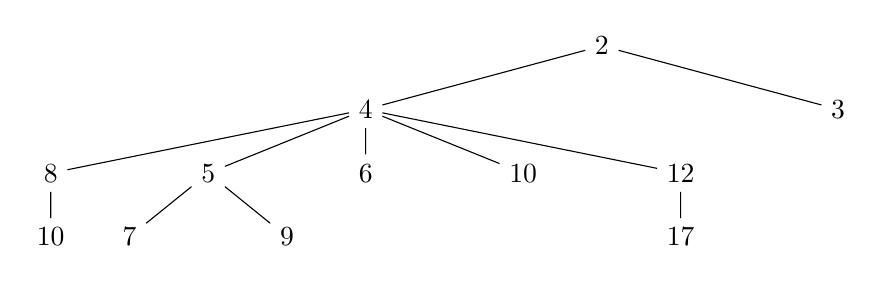
\begin{tikzpicture}[level 1/.style={sibling distance=60mm}, level 2/.style={sibling distance=20mm}, level distance=2.3em]
\node (2) {2}
  child {node (4) {4} %[sibling distance=20mm]
     child {node {8} child { node {10}}}
     child {node {5} child { node {7} } child { node {9}}}
     child {node {6} }
     child {node {10}}
     child {node {12} child { node {17}}}}
  child {node {3} };
\end{tikzpicture}
\end{center}
\end{frame}
%%%%%%%%%%%%%%%%%%%%%%%%%%%%%%%%%%%%%%%%%%%%%%%%%%%%%%%%%%%%%%%%%%%%%%%%%%%%%%%%%%%%



\section*{Handling Events}



%%%%%%%%%%%%%%%%%%%%%%%%%%%%%%%%%%%%%%%%%%%%%%%%%%%%%%%%%%%%%%%%%%%%%%%%%%%%%%%%%%%%
% Events and Finite-State Machines
%%%%%%%%%%%%%%%%%%%%%%%%%%%%%%%%%%%%%%%%%%%%%%%%%%%%%%%%%%%%%%%%%%%%%%%%%%%%%%%%%%%%
\begin{frame}{Events and Finite-State Machines}
Remember: reactive, not proactive.\vfill
How can the application do what it wants?\vfill
\Large Use \alert{Finite-State Machines}!
\uncover<2>{
\begin{center}
\scalebox{0.6}{
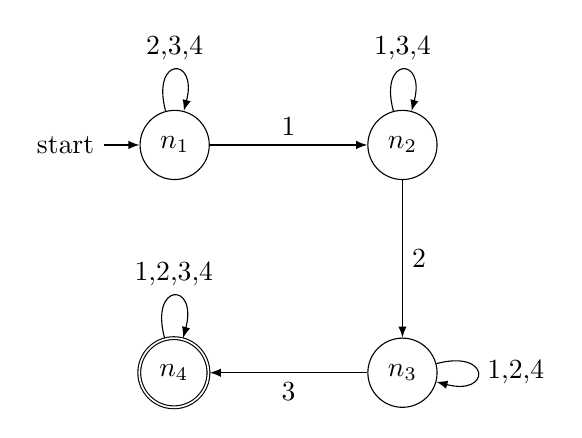
\begin{tikzpicture} [node distance=2cm, auto, every loop/.style={-latex},  every initial by arrow/.style={-latex}]

\node [state, initial] 	(n0){$n_1$};
\node [state] 			(n1) [right=of n0,]	{$n_2$};
\node [state]			(n2) [below=of n1]	{$n_3$};
\node [state, accepting](n3) [left=of n2]	{$n_4$};

\path[-latex] 
		(n0)edge				node	{1}		(n1)
			edge [loop above]	node	{2,3,4}	()
		(n1)edge				node	{2}		(n2)
			edge [loop above]	node	{1,3,4}	()
		(n2)edge				node	{3}		(n3)
			edge [loop right]	node	{1,2,4}	()
		(n3)edge [loop above]	node	{1,2,3,4}()
		;


\end{tikzpicture}}
\end{center}
}

\end{frame}
%%%%%%%%%%%%%%%%%%%%%%%%%%%%%%%%%%%%%%%%%%%%%%%%%%%%%%%%%%%%%%%%%%%%%%%%%%%%%%%%%%%%



\section*{Where Do Events Come From}



%%%%%%%%%%%%%%%%%%%%%%%%%%%%%%%%%%%%%%%%%%%%%%%%%%%%%%%%%%%%%%%%%%%%%%%%%%%%%%%%%%%%
% Where Events Come From
%%%%%%%%%%%%%%%%%%%%%%%%%%%%%%%%%%%%%%%%%%%%%%%%%%%%%%%%%%%%%%%%%%%%%%%%%%%%%%%%%%%%
\begin{frame}{Where Events Come From}
\begin{columns}
\begin{column}{0.5\textwidth}
\includegraphics[width=1.05\textwidth]{img/Galaxy_S_4G_037-small.png}

\vspace*{-1em}
\end{column}
\begin{column}{0.5\textwidth}
\uncover<2>{Analog-to-Digital Converter. Then what?}
\end{column}
\end{columns}

\end{frame}
%%%%%%%%%%%%%%%%%%%%%%%%%%%%%%%%%%%%%%%%%%%%%%%%%%%%%%%%%%%%%%%%%%%%%%%%%%%%%%%%%%%%



%%%%%%%%%%%%%%%%%%%%%%%%%%%%%%%%%%%%%%%%%%%%%%%%%%%%%%%%%%%%%%%%%%%%%%%%%%%%%%%%%%%%
% Where Events Come From
%%%%%%%%%%%%%%%%%%%%%%%%%%%%%%%%%%%%%%%%%%%%%%%%%%%%%%%%%%%%%%%%%%%%%%%%%%%%%%%%%%%%
\begin{frame}
\Huge
\begin{center}
``Are we there yet?''
\end{center}

\uncover<2>{\hfill --- example of \alert{polling}.}
\end{frame}
%%%%%%%%%%%%%%%%%%%%%%%%%%%%%%%%%%%%%%%%%%%%%%%%%%%%%%%%%%%%%%%%%%%%%%%%%%%%%%%%%%%%



%%%%%%%%%%%%%%%%%%%%%%%%%%%%%%%%%%%%%%%%%%%%%%%%%%%%%%%%%%%%%%%%%%%%%%%%%%%%%%%%%%%%
% Polling
%%%%%%%%%%%%%%%%%%%%%%%%%%%%%%%%%%%%%%%%%%%%%%%%%%%%%%%%%%%%%%%%%%%%%%%%%%%%%%%%%%%%
\begin{frame}{Polling}
\Large
\textbf{Polling:} processor requests readings from
the device at its convenience.  \vfill
``What is the current light level?''\vfill
(also known as ``passive synchronization'')
\end{frame}
%%%%%%%%%%%%%%%%%%%%%%%%%%%%%%%%%%%%%%%%%%%%%%%%%%%%%%%%%%%%%%%%%%%%%%%%%%%%%%%%%%%%



%%%%%%%%%%%%%%%%%%%%%%%%%%%%%%%%%%%%%%%%%%%%%%%%%%%%%%%%%%%%%%%%%%%%%%%%%%%%%%%%%%%%
% When to Poll?
%%%%%%%%%%%%%%%%%%%%%%%%%%%%%%%%%%%%%%%%%%%%%%%%%%%%%%%%%%%%%%%%%%%%%%%%%%%%%%%%%%%%
\begin{frame}{When to Poll?}
\large
It depends:

\begin{itemize}
\item whenever convenient (occasional polling);
\item at fixed time intervals (periodic polling); or
\item constantly (tight polling).
\end{itemize}
\end{frame}
%%%%%%%%%%%%%%%%%%%%%%%%%%%%%%%%%%%%%%%%%%%%%%%%%%%%%%%%%%%%%%%%%%%%%%%%%%%%%%%%%%%%



%%%%%%%%%%%%%%%%%%%%%%%%%%%%%%%%%%%%%%%%%%%%%%%%%%%%%%%%%%%%%%%%%%%%%%%%%%%%%%%%%%%%
% How to Get the Data
%%%%%%%%%%%%%%%%%%%%%%%%%%%%%%%%%%%%%%%%%%%%%%%%%%%%%%%%%%%%%%%%%%%%%%%%%%%%%%%%%%%%
\begin{frame}{How to Get the Data}
\vspace{1em}
\begin{center}
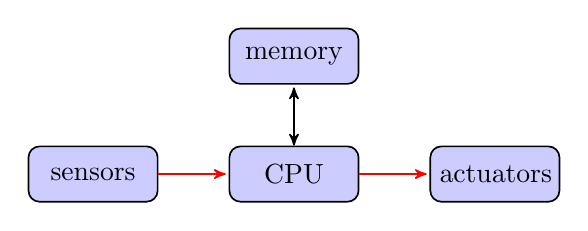
\begin{tikzpicture}[->,>=stealth',shorten >=1pt,auto,node distance=2.2cm,
                    semithick,initial text=]
  \node[bw]   (cpu)               {CPU};
  \node[bw, left of=cpu,xshift=-1em] (sensors) {sensors};
  \node[bw, right of=cpu,xshift=1em] (actuators) {actuators};
  \node[bw, above of=cpu,yshift=-2em] (memory) {memory};

  \path (cpu) edge[<->] node {} (memory)
        (sensors) edge[red] node {} (cpu)
        (cpu) edge[red] node {} (actuators);
\end{tikzpicture}
\end{center}

\large 
\vspace*{1em} What's the mechanism?

\uncover<2>{
\begin{itemize}
\item port-mapped I/O; or,\\[0.5em]
\item memory-mapped I/O
\end{itemize}
}
\end{frame}
%%%%%%%%%%%%%%%%%%%%%%%%%%%%%%%%%%%%%%%%%%%%%%%%%%%%%%%%%%%%%%%%%%%%%%%%%%%%%%%%%%%%



%%%%%%%%%%%%%%%%%%%%%%%%%%%%%%%%%%%%%%%%%%%%%%%%%%%%%%%%%%%%%%%%%%%%%%%%%%%%%%%%%%%%
% Port-mapped I/O: Special CPU Instructions
%%%%%%%%%%%%%%%%%%%%%%%%%%%%%%%%%%%%%%%%%%%%%%%%%%%%%%%%%%%%%%%%%%%%%%%%%%%%%%%%%%%%
\begin{frame}[fragile]{Port-mapped I/O: Special CPU Instructions}
The Intel ia32 processors provide special I/O instructions:\\[1em]
\begin{verbatim}
    outb   ax, 0x3f8
    inw    dx, ax
\end{verbatim}
~\\
May use a special bus, or set a specific signal on the bus.
\end{frame}
%%%%%%%%%%%%%%%%%%%%%%%%%%%%%%%%%%%%%%%%%%%%%%%%%%%%%%%%%%%%%%%%%%%%%%%%%%%%%%%%%%%%



%%%%%%%%%%%%%%%%%%%%%%%%%%%%%%%%%%%%%%%%%%%%%%%%%%%%%%%%%%%%%%%%%%%%%%%%%%%%%%%%%%%%
% Memory-mapped I/O Example
%%%%%%%%%%%%%%%%%%%%%%%%%%%%%%%%%%%%%%%%%%%%%%%%%%%%%%%%%%%%%%%%%%%%%%%%%%%%%%%%%%%%
\begin{frame}{Memory-mapped I/O Example}
\onslide<1->
{
\small
\begin{alltt}
 while (\alert{statusRegister} == 0x0000) \{\\
 \qquad // Do nothing until statusRegister changes value\\
 \}\\
 
 //  Read data that has changed from a dataRegister\\
 //  and store in memory\\
 incomingData = \alert{dataRegister};\\
\end{alltt}
}
\uncover<2>
{
\vspace{1em}
This is a \emph{tight polling loop}.
\begin{itemize}
\item Expect the hardware specification to promise that statusRegister eventually changes 
due to an external event.
\item Data exchange occurs once device is ready: \alert{polling synchronization}.
\end{itemize}
}
\end{frame}
%%%%%%%%%%%%%%%%%%%%%%%%%%%%%%%%%%%%%%%%%%%%%%%%%%%%%%%%%%%%%%%%%%%%%%%%%%%%%%%%%%%%



%%%%%%%%%%%%%%%%%%%%%%%%%%%%%%%%%%%%%%%%%%%%%%%%%%%%%%%%%%%%%%%%%%%%%%%%%%%%%%%%%%%%
% Interrupts: An Alternative Polling
%%%%%%%%%%%%%%%%%%%%%%%%%%%%%%%%%%%%%%%%%%%%%%%%%%%%%%%%%%%%%%%%%%%%%%%%%%%%%%%%%%%%
\begin{frame}{Interrupts: An Alternative Polling}
\large
So far: processor controls when to read data from a device.\vfill
Instead: device may tell the processor when device is ready,
using an \alert{interrupt}.\vfill
This constitutes \alert{active synchronization}.
\end{frame}
%%%%%%%%%%%%%%%%%%%%%%%%%%%%%%%%%%%%%%%%%%%%%%%%%%%%%%%%%%%%%%%%%%%%%%%%%%%%%%%%%%%%



%%%%%%%%%%%%%%%%%%%%%%%%%%%%%%%%%%%%%%%%%%%%%%%%%%%%%%%%%%%%%%%%%%%%%%%%%%%%%%%%%%%%
% How Interrupts Work
%%%%%%%%%%%%%%%%%%%%%%%%%%%%%%%%%%%%%%%%%%%%%%%%%%%%%%%%%%%%%%%%%%%%%%%%%%%%%%%%%%%%
\begin{frame}{How Interrupts Work}
Interrupt tells the processor: ``Something's happening!''\vfill

Upon receipt of an interrupt, the processor:
\begin{itemize}
\item stops what it's currently doing and saves its state;
\item starts executing pre-defined \alert{interrupt handler}, which:
\begin{itemize}
\item reads the event information; and
\item stores it somewhere accessible.
\end{itemize}
\item upon return from handler, resumes previous state.
\end{itemize}
\end{frame}
%%%%%%%%%%%%%%%%%%%%%%%%%%%%%%%%%%%%%%%%%%%%%%%%%%%%%%%%%%%%%%%%%%%%%%%%%%%%%%%%%%%%


\section*{Summing up: Inversion of Control}



%%%%%%%%%%%%%%%%%%%%%%%%%%%%%%%%%%%%%%%%%%%%%%%%%%%%%%%%%%%%%%%%%%%%%%%%%%%%%%%%%%%%
% Inversion of Control: Without It
%%%%%%%%%%%%%%%%%%%%%%%%%%%%%%%%%%%%%%%%%%%%%%%%%%%%%%%%%%%%%%%%%%%%%%%%%%%%%%%%%%%%
\begin{frame}{Inversion of Control: Without It}
Old ECE150 paradigm:\\[2em]

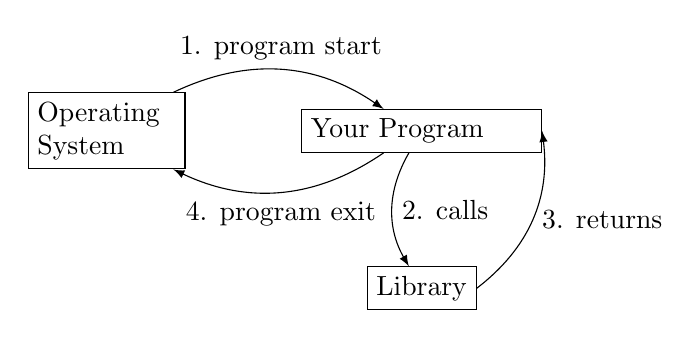
\begin{tikzpicture}
\path (0, 0) node[draw,text width=5em] (OS) { Operating System }
    +(4, 0) node[draw, text width=8em] (you) {Your Program};
\path<2-4> (4, -2) node[draw] (lib) {Library};

\path[->,bend left,>=latex] (OS) edge node[above] {1. program start} (you);
\path<4>[->,bend left,>=latex] (you) edge node[below] {4. program exit} (OS);
\path<2->[->,bend right,>=latex] (you) edge node[right] {2. calls} (lib);
\path<3->[->,bend right,>=latex] (lib.east) edge node[right] {3. returns} (you.east);
\end{tikzpicture}
\end{frame}
%%%%%%%%%%%%%%%%%%%%%%%%%%%%%%%%%%%%%%%%%%%%%%%%%%%%%%%%%%%%%%%%%%%%%%%%%%%%%%%%%%%%



%%%%%%%%%%%%%%%%%%%%%%%%%%%%%%%%%%%%%%%%%%%%%%%%%%%%%%%%%%%%%%%%%%%%%%%%%%%%%%%%%%%%
% Inversion of Control: With It
%%%%%%%%%%%%%%%%%%%%%%%%%%%%%%%%%%%%%%%%%%%%%%%%%%%%%%%%%%%%%%%%%%%%%%%%%%%%%%%%%%%%
\begin{frame}{Inversion of Control: With It}
New event-driven ECE155 paradigm:\\[2em]

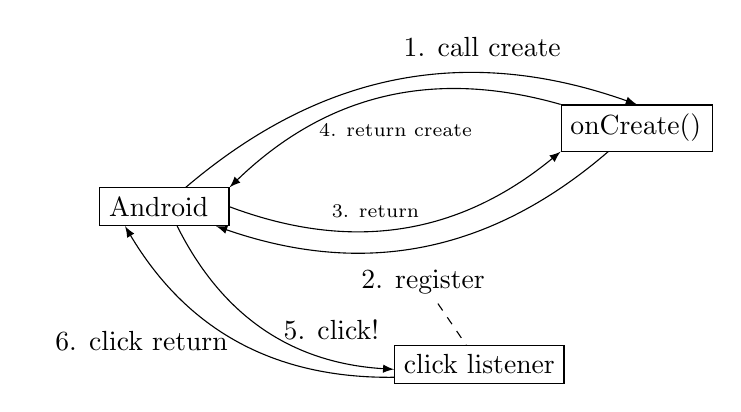
\begin{tikzpicture}
\path (0, 0) node[draw,text width=4em] (OS) { Android }
    +(6, 1) node[draw, text width=4.8em] (you) { onCreate() };
\path<2-> (4, -2) node[draw] (listener) {click listener};

\path[->,bend left,>=latex] (OS) edge node[above,yshift=0.5em, xshift=3em] {1. call create} (you.north);
\path<2->[->,bend left,>=latex] (you) edge node[below,name=reg,yshift=-.5em] {2. register} (OS);
\path<2->[dashed] (reg) edge (listener);
\path<3->[<-,bend left,>=latex] (you.south west) edge node[above,xshift=-1em,name=reg] {\scriptsize 3. return} (OS.east);
\path<4->[->,bend right,>=latex] (you.north west) edge node[above,at end,xshift=6em,yshift=1.5em] {\scriptsize 4. return create} (OS.north east);
\path<5->[->,bend right,>=latex] (OS) edge node[right] {~5. click!} (listener);
\path<6->[<-,bend right,>=latex] (OS.south)+(-0.5,0) edge node[left] {~~6. click return} 
                                 (listener)+(1,0);
\end{tikzpicture}
\end{frame}
%%%%%%%%%%%%%%%%%%%%%%%%%%%%%%%%%%%%%%%%%%%%%%%%%%%%%%%%%%%%%%%%%%%%%%%%%%%%%%%%%%%%



%%%%%%%%%%%%%%%%%%%%%%%%%%%%%%%%%%%%%%%%%%%%%%%%%%%%%%%%%%%%%%%%%%%%%%%%%%%%%%%%%%%%
% Behind the Scenes for Inversion of Control
%%%%%%%%%%%%%%%%%%%%%%%%%%%%%%%%%%%%%%%%%%%%%%%%%%%%%%%%%%%%%%%%%%%%%%%%%%%%%%%%%%%%
\begin{frame}[fragile]{Behind the Scenes for Inversion of Control}
Android is running an event loop for each thread:
\begin{verbatim}
while (!done) {
 r <- fetch Runnable from Queue
 dispatch r
}
\end{verbatim}
This is a polling loop: in particular, a \structure{tight polling loop}, but which
goes to sleep waiting for the next event (in fetch).
\end{frame}
%%%%%%%%%%%%%%%%%%%%%%%%%%%%%%%%%%%%%%%%%%%%%%%%%%%%%%%%%%%%%%%%%%%%%%%%%%%%%%%%%%%%



%%%%%%%%%%%%%%%%%%%%%%%%%%%%%%%%%%%%%%%%%%%%%%%%%%%%%%%%%%%%%%%%%%%%%%%%%%%%%%%%%%%%
% Miscellaneous: Real-Time Systems
%%%%%%%%%%%%%%%%%%%%%%%%%%%%%%%%%%%%%%%%%%%%%%%%%%%%%%%%%%%%%%%%%%%%%%%%%%%%%%%%%%%%
\begin{frame}{Miscellaneous: Real-Time Systems}
Must respond to an external event in a fixed amount of time. \\[1em]

This fixed amount of time is not necessarily small.
\begin{itemize}
\item may potentially be fixed and large.
\end{itemize}

Many embedded systems must satisfy real-time constraints.\\[1em]

In upper-year courses, you'll see both embedded systems and real-time
systems in more detail.

\end{frame}
%%%%%%%%%%%%%%%%%%%%%%%%%%%%%%%%%%%%%%%%%%%%%%%%%%%%%%%%%%%%%%%%%%%%%%%%%%%%%%%%%%%%



%%%%%%%%%%%%%%%%%%%%%%%%%%%%%%%%%%%%%%%%%%%%%%%%%%%%%%%%%%%%%%%%%%%%%%%%%%%%%%%%%%%%
% Real-Time System Example
%%%%%%%%%%%%%%%%%%%%%%%%%%%%%%%%%%%%%%%%%%%%%%%%%%%%%%%%%%%%%%%%%%%%%%%%%%%%%%%%%%%%
\begin{frame}{Real-Time System Example}
\begin{center}
\includegraphics[height=0.4\textheight]{img/bluray}
\end{center}
\hfill {\tiny (credit {\tt digitaljournal.com}, from flickr)} \\
Blu-Ray player must:
\begin{itemize}
\item read compressed video data from a media disk;
\item decompress the video; and
\item output it to a HDMI interface,
\end{itemize}
all within a fixed amount of time, to avoid a degradation of video quality.
\end{frame}
%%%%%%%%%%%%%%%%%%%%%%%%%%%%%%%%%%%%%%%%%%%%%%%%%%%%%%%%%%%%%%%%%%%%%%%%%%%%%%%%%%%%


\section*{Demo: Android Sensor Manager}



\end{document}